\documentclass[12pt,a4paper,times]{report}
\usepackage[utf8]{inputenc}
\usepackage[english]{babel}
\usepackage{amsmath}
\usepackage{amsfonts}
\usepackage{amssymb}
\usepackage{amsthm}
\usepackage{bm}
\usepackage[font=small, labelfont=bf]{caption}
\usepackage{xcolor}
\usepackage{csquotes}
\usepackage{enumerate}
\usepackage{faktor}
\usepackage{graphicx}
\usepackage{hyperref}
\usepackage{mathrsfs}
\usepackage{mathtools}
\usepackage{pgf,tikz}
\usepackage{pgfplots, pgfplotstable}
\usepackage{showlabels}
\usepackage{tikz-cd}
\usepackage{url}
\usepackage{times}

\usepackage{biblatex}
\addbibresource{bibliography.bib}

\pgfplotsset{compat=1.18}
\usetikzlibrary{arrows}
\usetikzlibrary{decorations.pathreplacing,decorations.markings}

\numberwithin{equation}{section}
\numberwithin{figure}{section}

\newtheorem{lemma}{Lemma}[section]
\numberwithin{lemma}{section}
\newtheorem{corollary}[lemma]{Corollary}
\newtheorem{proposition}[lemma]{Proposition}
\newtheorem{theorem}[lemma]{Theorem}

\theoremstyle{definition}
\newtheorem{assumption}[lemma]{Assumption}
\newtheorem{definition}[lemma]{Definition}
\newtheorem{example}[lemma]{Example}
\newtheorem{remark}[lemma]{Remark}
\newtheorem{problem}[lemma]{Problem}

\DeclareMathOperator{\ad}{ad}
\DeclareMathOperator{\alt}{Alt}
\DeclareMathOperator*{\esssup}{ess\,sup}
\DeclareMathOperator{\curl}{curl}
\DeclareMathOperator{\diver}{div}
\DeclareMathOperator{\gap}{gap}
\DeclareMathOperator{\grad}{grad}
\DeclareMathOperator{\Id}{Id}
\DeclareMathOperator{\Ima}{im}
\DeclareMathOperator{\interior}{int}
\DeclareMathOperator{\sgn}{sgn}
\DeclareMathOperator{\spanvec}{span}
\DeclareMathOperator{\supp}{supp}
\DeclareMathOperator{\tr}{tr}
\DeclareMathOperator{\vol}{vol}

\newcommand{\aop}{\mathscr{A}}
\newcommand{\alternating}[2]{ {\alt^{#1}\,#2} }
\newcommand{\integers}{\mathbb{Z}}
\newcommand{\smoothcompforms}[2]{C_c^\infty \Lambda^{#1}(#2)}
\newcommand{\lpcoho}{H^k_{p,dR}}
\newcommand{\naturalnum}{\mathbb{N}}
\newcommand{\norm}[2]{\lVert #1 \rVert_{#2}}
\newcommand{\omegabar}{\overline{\Omega}}
\newcommand{\rational}{\mathbb{Q}}
\newcommand{\real}{\mathbb{R}}
\newcommand{\rop}{\mathscr{R}} % short for R operator
\newcommand{\veccurl}{\bm{\curl}}
\newcommand{\weakcurl}{\widetilde{\curl}}

\usepackage{subfiles}

\begin{document}
\pagenumbering{roman}
\begin{titlepage}
    \begin{center}
    
\includegraphics[width=0.18\textwidth]{img/tum.png}\par
    \vspace{0.5cm}
    {\scshape\LARGE Technical University Munich \par}
    \vspace{0.5cm}
    {\scshape \Large Department of Mathematics\par}
    \vspace{1cm}
	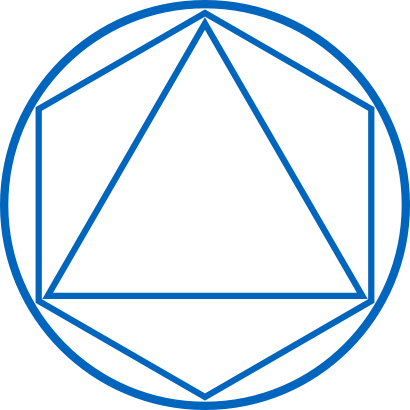
\includegraphics[width=0.25\textwidth]{img/ma_tum.png}\par
    \vspace{0.5cm}
    {\scshape \LARGE Master's Thesis \par}
    \vspace{0.6cm}
   {\Huge \scshape The Magnetostatic Problem on Exterior Domains \par}
   \vspace{0.7cm}
   
   {\scshape \Large Alexander Hoffmann\par}
   

	\end{center}
	\vfill
    Supervisor: PD Dr. Martin Campos Pinto
    \medskip
    
    \noindent Advisor: PD Dr. Martin Campos Pinto
    \medskip
    
    \noindent Submission Date: 15.08.2023
    \vspace{1cm}
\end{titlepage}
%FOR THE PRINT!
\
\thispagestyle{empty}
\newpage

%empty page
%BEGIN_FOLD
\ {}
\vfill
\thispagestyle{empty}
\noindent I assure the single handed composition of this master's thesis is only supported by declared resources.
\bigskip

\noindent München, August 13, 2023 \par
\vspace{2,5cm}
 
\noindent\hspace{1cm} Alexander Hoffmann
    \vspace{1cm}
\newpage
\thispagestyle{empty}
%zusammenfassung in deutscher Sprache
% \belowpdfbookmark{Abstract}{abstract}
\section*{Zusammenfassung}
\subfile{abstract/german/abstract.tex}
\vspace{1cm}
\section*{Summary}
\subfile{abstract/english/abstract.tex}
\newpage

\thispagestyle{empty}
%zusammenfassung in deutscher Sprache
% \belowpdfbookmark{Abstract}{abstract}
\section*{Acknowledgements}
I would like to thank Martin Campos Pinto for investing a lot of his time 
to provide suggestions, guidance and ideas without which this thesis would not have 
been possible. I also want to thank Omar Maj and Florian Hindenlang for answering questions regarding the physics 
and Yaman Güçlü for helping with the implementation. Additionally, I would like to take 
this opportunity to express my gratitude to my parents without whose support I would have 
been unable to dedicate as much time to this thesis as I did.
\newpage

\tableofcontents
\newpage
\pagenumbering{arabic}
\setcounter{page}{1}

\chapter*{Introduction}\label{chap:introduction}
\subfile{introduction/introduction.tex}
\chapter{Existence and uniqueness}\label{chap:existence_and_uniqueness}
\subfile{part1/Part1.tex}
\chapter{Numerical approximation in 2D}\label{chap:approximation_in_2D}
\subfile{part2/part2.tex}
\chapter{Conclusion and Further Directions}\label{chap:conclusion}
\subfile{conclusion/conclusion.tex}
\printbibliography
\end{document}